\documentclass[1p]{elsarticle_modified}
%\bibliographystyle{elsarticle-num}

%\usepackage[colorlinks]{hyperref}
%\usepackage{abbrmath_seonhwa} %\Abb, \Ascr, \Acal ,\Abf, \Afrak
\usepackage{amsfonts}
\usepackage{amssymb}
\usepackage{amsmath}
\usepackage{amsthm}
\usepackage{scalefnt}
\usepackage{amsbsy}
\usepackage{kotex}
\usepackage{caption}
\usepackage{subfig}
\usepackage{color}
\usepackage{graphicx}
\usepackage{xcolor} %% white, black, red, green, blue, cyan, magenta, yellow
\usepackage{float}
\usepackage{setspace}
\usepackage{hyperref}

\usepackage{tikz}
\usetikzlibrary{arrows}

\usepackage{multirow}
\usepackage{array} % fixed length table
\usepackage{hhline}

%%%%%%%%%%%%%%%%%%%%%
\makeatletter
\renewcommand*\env@matrix[1][\arraystretch]{%
	\edef\arraystretch{#1}%
	\hskip -\arraycolsep
	\let\@ifnextchar\new@ifnextchar
	\array{*\c@MaxMatrixCols c}}
\makeatother %https://tex.stackexchange.com/questions/14071/how-can-i-increase-the-line-spacing-in-a-matrix
%%%%%%%%%%%%%%%

\usepackage[normalem]{ulem}

\newcommand{\msout}[1]{\ifmmode\text{\sout{\ensuremath{#1}}}\else\sout{#1}\fi}
%SOURCE: \msout is \stkout macro in https://tex.stackexchange.com/questions/20609/strikeout-in-math-mode

\newcommand{\cancel}[1]{
	\ifmmode
	{\color{red}\msout{#1}}
	\else
	{\color{red}\sout{#1}}
	\fi
}

\newcommand{\add}[1]{
	{\color{blue}\uwave{#1}}
}

\newcommand{\replace}[2]{
	\ifmmode
	{\color{red}\msout{#1}}{\color{blue}\uwave{#2}}
	\else
	{\color{red}\sout{#1}}{\color{blue}\uwave{#2}}
	\fi
}

\newcommand{\Sol}{\mathcal{S}} %segment
\newcommand{\D}{D} %diagram
\newcommand{\A}{\mathcal{A}} %arc


%%%%%%%%%%%%%%%%%%%%%%%%%%%%%5 test

\def\sl{\operatorname{\textup{SL}}(2,\Cbb)}
\def\psl{\operatorname{\textup{PSL}}(2,\Cbb)}
\def\quan{\mkern 1mu \triangleright \mkern 1mu}

\theoremstyle{definition}
\newtheorem{thm}{Theorem}[section]
\newtheorem{prop}[thm]{Proposition}
\newtheorem{lem}[thm]{Lemma}
\newtheorem{ques}[thm]{Question}
\newtheorem{cor}[thm]{Corollary}
\newtheorem{defn}[thm]{Definition}
\newtheorem{exam}[thm]{Example}
\newtheorem{rmk}[thm]{Remark}
\newtheorem{alg}[thm]{Algorithm}

\newcommand{\I}{\sqrt{-1}}
\begin{document}

%\begin{frontmatter}
%
%\title{Boundary parabolic representations of knots up to 8 crossings}
%
%%% Group authors per affiliation:
%\author{Yunhi Cho} 
%\address{Department of Mathematics, University of Seoul, Seoul, Korea}
%\ead{yhcho@uos.ac.kr}
%
%
%\author{Seonhwa Kim} %\fnref{s_kim}}
%\address{Center for Geometry and Physics, Institute for Basic Science, Pohang, 37673, Korea}
%\ead{ryeona17@ibs.re.kr}
%
%\author{Hyuk Kim}
%\address{Department of Mathematical Sciences, Seoul National University, Seoul 08826, Korea}
%\ead{hyukkim@snu.ac.kr}
%
%\author{Seokbeom Yoon}
%\address{Department of Mathematical Sciences, Seoul National University, Seoul, 08826,  Korea}
%\ead{sbyoon15@snu.ac.kr}
%
%\begin{abstract}
%We find all boundary parabolic representation of knots up to 8 crossings.
%
%\end{abstract}
%\begin{keyword}
%    \MSC[2010] 57M25 
%\end{keyword}
%
%\end{frontmatter}

%\linenumbers
%\tableofcontents
%
\newcommand\colored[1]{\textcolor{white}{\rule[-0.35ex]{0.8em}{1.4ex}}\kern-0.8em\color{red} #1}%
%\newcommand\colored[1]{\textcolor{white}{ #1}\kern-2.17ex	\textcolor{white}{ #1}\kern-1.81ex	\textcolor{white}{ #1}\kern-2.15ex\color{red}#1	}

{\Large $\underline{12a_{0056}~(K12a_{0056})}$}

\setlength{\tabcolsep}{10pt}
\renewcommand{\arraystretch}{1.6}
\vspace{1cm}\begin{tabular}{m{100pt}>{\centering\arraybackslash}m{274pt}}
\multirow{5}{120pt}{
	\centering
	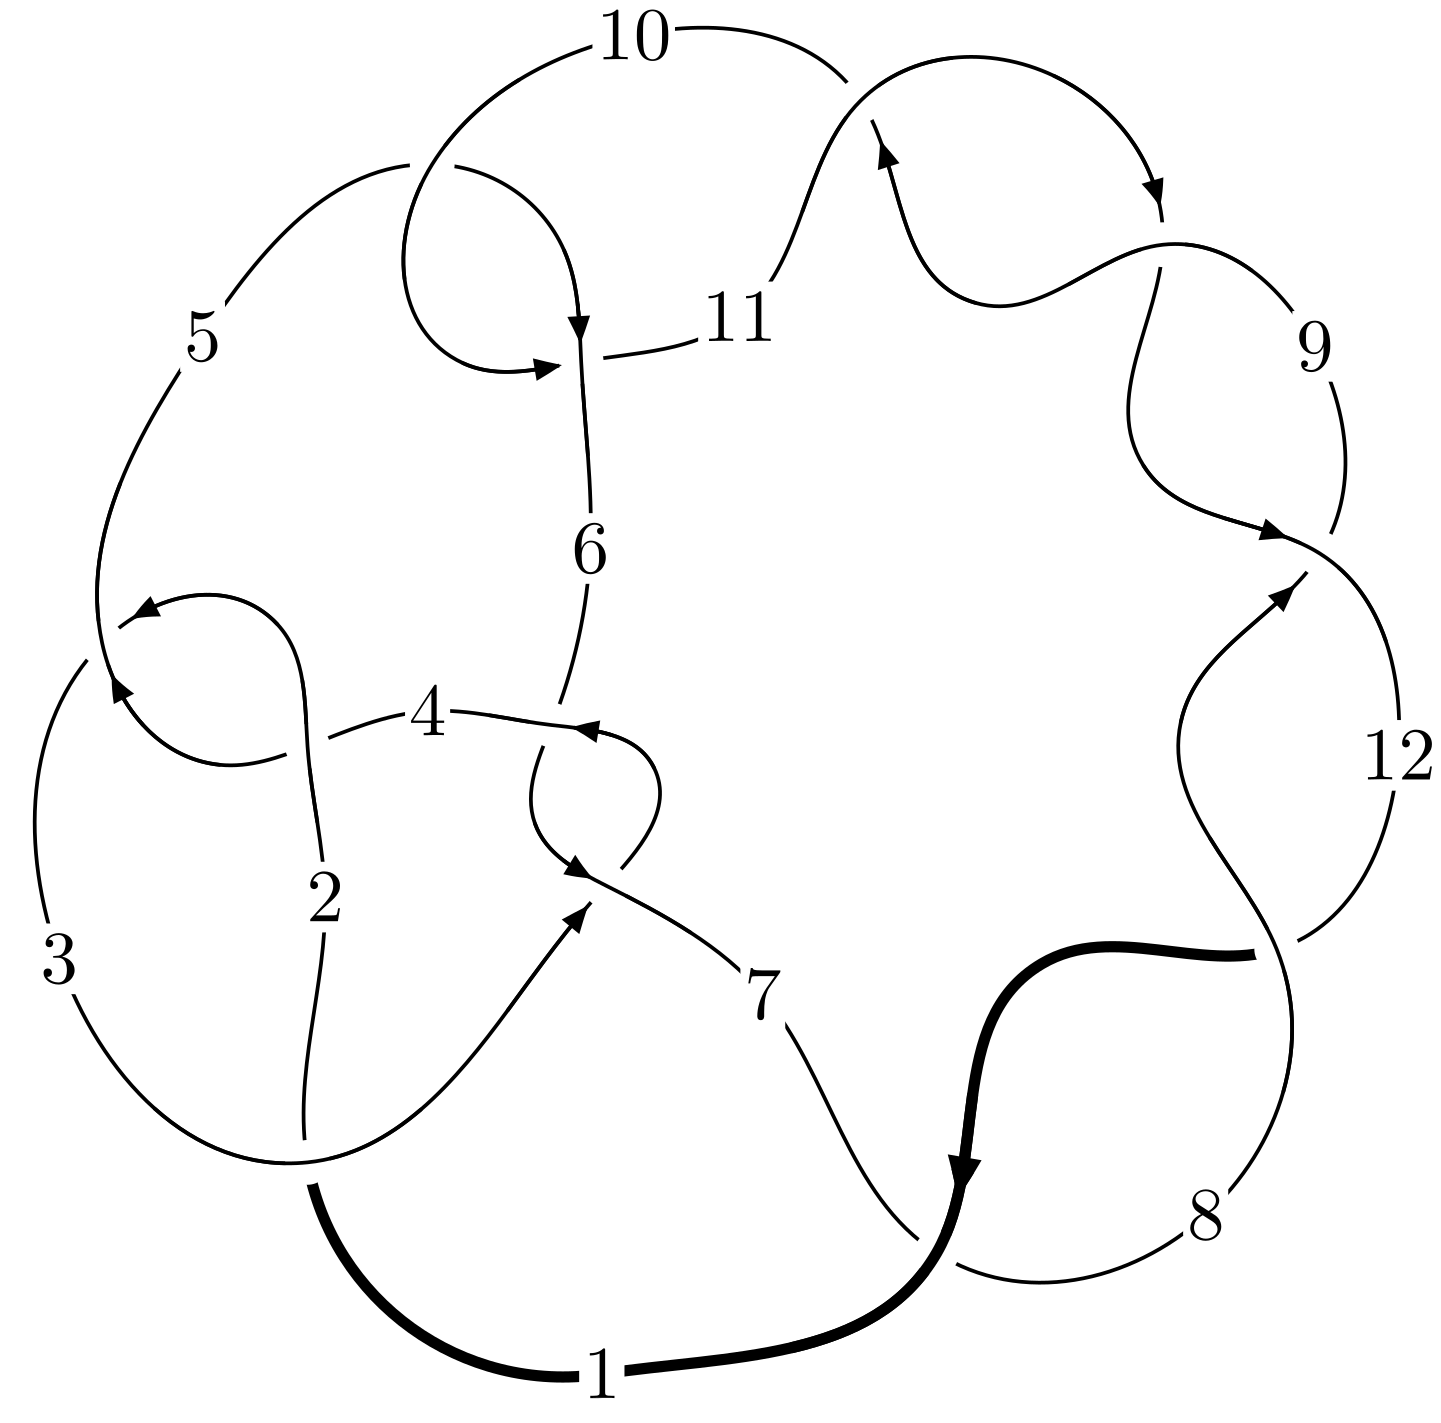
\includegraphics[width=112pt]{../../../GIT/diagram.site/Diagrams/png/857_12a_0056.png}\\
\ \ \ A knot diagram\footnotemark}&
\allowdisplaybreaks
\textbf{Linearized knot diagam} \\
\cline{2-2}
 &
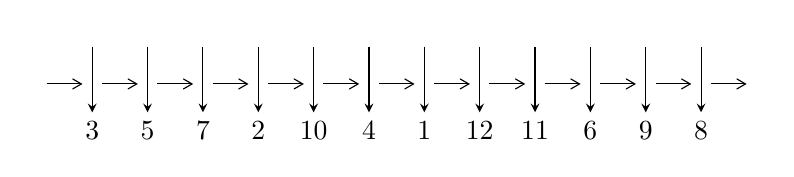
\begin{tikzpicture}[x=20pt, y=17pt]
	% nodes
	\node (C0) at (0, 0) {};
	\node (C1) at (1, 0) {};
	\node (C1U) at (1, +1) {};
	\node (C1D) at (1, -1) {3};

	\node (C2) at (2, 0) {};
	\node (C2U) at (2, +1) {};
	\node (C2D) at (2, -1) {5};

	\node (C3) at (3, 0) {};
	\node (C3U) at (3, +1) {};
	\node (C3D) at (3, -1) {7};

	\node (C4) at (4, 0) {};
	\node (C4U) at (4, +1) {};
	\node (C4D) at (4, -1) {2};

	\node (C5) at (5, 0) {};
	\node (C5U) at (5, +1) {};
	\node (C5D) at (5, -1) {10};

	\node (C6) at (6, 0) {};
	\node (C6U) at (6, +1) {};
	\node (C6D) at (6, -1) {4};

	\node (C7) at (7, 0) {};
	\node (C7U) at (7, +1) {};
	\node (C7D) at (7, -1) {1};

	\node (C8) at (8, 0) {};
	\node (C8U) at (8, +1) {};
	\node (C8D) at (8, -1) {12};

	\node (C9) at (9, 0) {};
	\node (C9U) at (9, +1) {};
	\node (C9D) at (9, -1) {11};

	\node (C10) at (10, 0) {};
	\node (C10U) at (10, +1) {};
	\node (C10D) at (10, -1) {6};

	\node (C11) at (11, 0) {};
	\node (C11U) at (11, +1) {};
	\node (C11D) at (11, -1) {9};

	\node (C12) at (12, 0) {};
	\node (C12U) at (12, +1) {};
	\node (C12D) at (12, -1) {8};
	\node (C13) at (13, 0) {};

	% arrows
	\draw[->,>={angle 60}]
	(C0) edge (C1) (C1) edge (C2) (C2) edge (C3) (C3) edge (C4) (C4) edge (C5) (C5) edge (C6) (C6) edge (C7) (C7) edge (C8) (C8) edge (C9) (C9) edge (C10) (C10) edge (C11) (C11) edge (C12) (C12) edge (C13) ;	\draw[->,>=stealth]
	(C1U) edge (C1D) (C2U) edge (C2D) (C3U) edge (C3D) (C4U) edge (C4D) (C5U) edge (C5D) (C6U) edge (C6D) (C7U) edge (C7D) (C8U) edge (C8D) (C9U) edge (C9D) (C10U) edge (C10D) (C11U) edge (C11D) (C12U) edge (C12D) ;
	\end{tikzpicture} \\
\hhline{~~} \\& 
\textbf{Solving Sequence} \\ \cline{2-2} 
 &
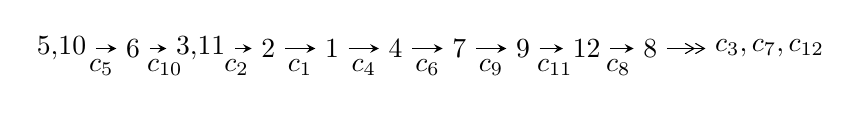
\begin{tikzpicture}[x=23pt, y=7pt]
	% node
	\node (A0) at (-1/8, 0) {5,10};
	\node (A1) at (1, 0) {6};
	\node (A2) at (33/16, 0) {3,11};
	\node (A3) at (25/8, 0) {2};
	\node (A4) at (33/8, 0) {1};
	\node (A5) at (41/8, 0) {4};
	\node (A6) at (49/8, 0) {7};
	\node (A7) at (57/8, 0) {9};
	\node (A8) at (65/8, 0) {12};
	\node (A9) at (73/8, 0) {8};
	\node (C1) at (1/2, -1) {$c_{5}$};
	\node (C2) at (3/2, -1) {$c_{10}$};
	\node (C3) at (21/8, -1) {$c_{2}$};
	\node (C4) at (29/8, -1) {$c_{1}$};
	\node (C5) at (37/8, -1) {$c_{4}$};
	\node (C6) at (45/8, -1) {$c_{6}$};
	\node (C7) at (53/8, -1) {$c_{9}$};
	\node (C8) at (61/8, -1) {$c_{11}$};
	\node (C9) at (69/8, -1) {$c_{8}$};
	\node (A10) at (11, 0) {$c_{3},c_{7},c_{12}$};

	% edge
	\draw[->,>=stealth]	
	(A0) edge (A1) (A1) edge (A2) (A2) edge (A3) (A3) edge (A4) (A4) edge (A5) (A5) edge (A6) (A6) edge (A7) (A7) edge (A8) (A8) edge (A9) ;
	\draw[->>,>={angle 60}]	
	(A9) edge (A10);
\end{tikzpicture} \\ 

\end{tabular} \\

\footnotetext{
The image of knot diagram is generated by the software ``\textbf{Draw programme}" developed by Andrew Bartholomew(\url{http://www.layer8.co.uk/maths/draw/index.htm\#Running-draw}), where we modified some parts for our purpose(\url{https://github.com/CATsTAILs/LinksPainter}).
}\phantom \\ \newline 
\centering \textbf{Ideals for irreducible components\footnotemark of $X_{\text{par}}$} 
 
\begin{align*}
I^u_{1}&=\langle 
- u^{48}- u^{47}+\cdots+b+1,\;u^{45}-4 u^{43}+\cdots+a-5 u,\;u^{49}+2 u^{48}+\cdots+u-1\rangle \\
I^u_{2}&=\langle 
b+1,\;u^4- u^2+a+u+2,\;u^5- u^4+u^2+u-1\rangle \\
\\
\end{align*}
\raggedright * 2 irreducible components of $\dim_{\mathbb{C}}=0$, with total 54 representations.\\
\footnotetext{All coefficients of polynomials are rational numbers. But the coefficients are sometimes approximated in decimal forms when there is not enough margin.}
\newpage
\renewcommand{\arraystretch}{1}
\centering \section*{I. $I^u_{1}= \langle - u^{48}- u^{47}+\cdots+b+1,\;u^{45}-4 u^{43}+\cdots+a-5 u,\;u^{49}+2 u^{48}+\cdots+u-1 \rangle$}
\flushleft \textbf{(i) Arc colorings}\\
\begin{tabular}{m{7pt} m{180pt} m{7pt} m{180pt} }
\flushright $a_{5}=$&$\begin{pmatrix}1\\0\end{pmatrix}$ \\
\flushright $a_{10}=$&$\begin{pmatrix}0\\u\end{pmatrix}$ \\
\flushright $a_{6}=$&$\begin{pmatrix}1\\u^2\end{pmatrix}$ \\
\flushright $a_{3}=$&$\begin{pmatrix}- u^{45}+4 u^{43}+\cdots-22 u^3+5 u\\u^{48}+u^{47}+\cdots+4 u^2-1\end{pmatrix}$ \\
\flushright $a_{11}=$&$\begin{pmatrix}- u\\- u^3+u\end{pmatrix}$ \\
\flushright $a_{2}=$&$\begin{pmatrix}u^{48}+u^{47}+\cdots+5 u-1\\u^{48}+u^{47}+\cdots+4 u^2-1\end{pmatrix}$ \\
\flushright $a_{1}=$&$\begin{pmatrix}u^9+3 u^5+u\\u^{11}- u^9+4 u^7-3 u^5+3 u^3- u\end{pmatrix}$ \\
\flushright $a_{4}=$&$\begin{pmatrix}2 u^{48}+2 u^{47}+\cdots+6 u-1\\u^{48}+u^{47}+\cdots+u-1\end{pmatrix}$ \\
\flushright $a_{7}=$&$\begin{pmatrix}u^{11}+4 u^7+3 u^3\\u^{13}- u^{11}+5 u^9-4 u^7+6 u^5-3 u^3+u\end{pmatrix}$ \\
\flushright $a_{9}=$&$\begin{pmatrix}u^3\\u^5- u^3+u\end{pmatrix}$ \\
\flushright $a_{12}=$&$\begin{pmatrix}- u^5- u\\- u^7+u^5-2 u^3+u\end{pmatrix}$ \\
\flushright $a_{8}=$&$\begin{pmatrix}u^7+2 u^3\\u^9- u^7+3 u^5-2 u^3+u\end{pmatrix}$\\&\end{tabular}
\flushleft \textbf{(ii) Obstruction class $= -1$}\\~\\
\flushleft \textbf{(iii) Cusp Shapes $= 6 u^{48}+5 u^{47}+\cdots+9 u-20$}\\~\\
\newpage\renewcommand{\arraystretch}{1}
\flushleft \textbf{(iv) u-Polynomials at the component}\newline \\
\begin{tabular}{m{50pt}|m{274pt}}
Crossings & \hspace{64pt}u-Polynomials at each crossing \\
\hline $$\begin{aligned}c_{1}\end{aligned}$$&$\begin{aligned}
&u^{49}+20 u^{48}+\cdots+79 u+1
\end{aligned}$\\
\hline $$\begin{aligned}c_{2},c_{4}\end{aligned}$$&$\begin{aligned}
&u^{49}-6 u^{48}+\cdots- u+1
\end{aligned}$\\
\hline $$\begin{aligned}c_{3},c_{6}\end{aligned}$$&$\begin{aligned}
&u^{49}- u^{48}+\cdots+64 u+32
\end{aligned}$\\
\hline $$\begin{aligned}c_{5},c_{10}\end{aligned}$$&$\begin{aligned}
&u^{49}-2 u^{48}+\cdots+u+1
\end{aligned}$\\
\hline $$\begin{aligned}c_{7},c_{8},c_{9}\\c_{11},c_{12}\end{aligned}$$&$\begin{aligned}
&u^{49}+8 u^{48}+\cdots+13 u+1
\end{aligned}$\\
\hline
\end{tabular}\\~\\
\newpage\renewcommand{\arraystretch}{1}
\flushleft \textbf{(v) Riley Polynomials at the component}\newline \\
\begin{tabular}{m{50pt}|m{274pt}}
Crossings & \hspace{64pt}Riley Polynomials at each crossing \\
\hline $$\begin{aligned}c_{1}\end{aligned}$$&$\begin{aligned}
&y^{49}+24 y^{48}+\cdots+2991 y-1
\end{aligned}$\\
\hline $$\begin{aligned}c_{2},c_{4}\end{aligned}$$&$\begin{aligned}
&y^{49}-20 y^{48}+\cdots+79 y-1
\end{aligned}$\\
\hline $$\begin{aligned}c_{3},c_{6}\end{aligned}$$&$\begin{aligned}
&y^{49}+33 y^{48}+\cdots-9728 y-1024
\end{aligned}$\\
\hline $$\begin{aligned}c_{5},c_{10}\end{aligned}$$&$\begin{aligned}
&y^{49}-8 y^{48}+\cdots+13 y-1
\end{aligned}$\\
\hline $$\begin{aligned}c_{7},c_{8},c_{9}\\c_{11},c_{12}\end{aligned}$$&$\begin{aligned}
&y^{49}+68 y^{48}+\cdots-67 y-1
\end{aligned}$\\
\hline
\end{tabular}\\~\\
\newpage\flushleft \textbf{(vi) Complex Volumes and Cusp Shapes}
$$\begin{array}{c|c|c}  
\text{Solutions to }I^u_{1}& \I (\text{vol} + \sqrt{-1}CS) & \text{Cusp shape}\\
 \hline 
\begin{aligned}
u &= -0.760736 + 0.719246 I \\
a &= \phantom{-}1.12247 + 1.09140 I \\
b &= -0.784658 - 0.558197 I\end{aligned}
 & \phantom{-}3.14913 + 0.38825 I & -7.13985 + 0. I\phantom{ +0.000000I} \\ \hline\begin{aligned}
u &= -0.760736 - 0.719246 I \\
a &= \phantom{-}1.12247 - 1.09140 I \\
b &= -0.784658 + 0.558197 I\end{aligned}
 & \phantom{-}3.14913 - 0.38825 I & -7.13985 + 0. I\phantom{ +0.000000I} \\ \hline\begin{aligned}
u &= \phantom{-}0.796734 + 0.681722 I \\
a &= -0.291180 + 1.036890 I \\
b &= -1.281700 + 0.033312 I\end{aligned}
 & \phantom{-}1.51702 - 2.54299 I & -6.23264 + 3.96997 I \\ \hline\begin{aligned}
u &= \phantom{-}0.796734 - 0.681722 I \\
a &= -0.291180 - 1.036890 I \\
b &= -1.281700 - 0.033312 I\end{aligned}
 & \phantom{-}1.51702 + 2.54299 I & -6.23264 - 3.96997 I \\ \hline\begin{aligned}
u &= -0.892137 + 0.327379 I \\
a &= \phantom{-}2.17207 + 1.31935 I \\
b &= \phantom{-}1.005090 - 0.623169 I\end{aligned}
 & \phantom{-}0.43580 + 6.91892 I & -11.9536 - 9.3736 I \\ \hline\begin{aligned}
u &= -0.892137 - 0.327379 I \\
a &= \phantom{-}2.17207 - 1.31935 I \\
b &= \phantom{-}1.005090 + 0.623169 I\end{aligned}
 & \phantom{-}0.43580 - 6.91892 I & -11.9536 + 9.3736 I \\ \hline\begin{aligned}
u &= -0.844082 + 0.428322 I \\
a &= -0.187763 + 0.837953 I \\
b &= \phantom{-}0.617924 + 0.579853 I\end{aligned}
 & \phantom{-}1.59253 + 2.02971 I & -8.12894 - 3.92342 I \\ \hline\begin{aligned}
u &= -0.844082 - 0.428322 I \\
a &= -0.187763 - 0.837953 I \\
b &= \phantom{-}0.617924 - 0.579853 I\end{aligned}
 & \phantom{-}1.59253 - 2.02971 I & -8.12894 + 3.92342 I \\ \hline\begin{aligned}
u &= \phantom{-}0.693592 + 0.795699 I \\
a &= -0.527393 + 1.026490 I \\
b &= \phantom{-}1.070340 - 0.723216 I\end{aligned}
 & \phantom{-}7.01029 + 5.24368 I & -5.42899 - 3.02603 I \\ \hline\begin{aligned}
u &= \phantom{-}0.693592 - 0.795699 I \\
a &= -0.527393 - 1.026490 I \\
b &= \phantom{-}1.070340 + 0.723216 I\end{aligned}
 & \phantom{-}7.01029 - 5.24368 I & -5.42899 + 3.02603 I\\
 \hline 
 \end{array}$$\newpage$$\begin{array}{c|c|c}  
\text{Solutions to }I^u_{1}& \I (\text{vol} + \sqrt{-1}CS) & \text{Cusp shape}\\
 \hline 
\begin{aligned}
u &= -0.842140 + 0.687789 I \\
a &= -0.05555 - 2.42181 I \\
b &= -0.868271 + 0.553100 I\end{aligned}
 & \phantom{-}2.88211 + 4.83632 I & -8.23420 - 6.42667 I \\ \hline\begin{aligned}
u &= -0.842140 - 0.687789 I \\
a &= -0.05555 + 2.42181 I \\
b &= -0.868271 - 0.553100 I\end{aligned}
 & \phantom{-}2.88211 - 4.83632 I & -8.23420 + 6.42667 I \\ \hline\begin{aligned}
u &= \phantom{-}0.749509 + 0.792916 I \\
a &= -0.060126 - 1.378320 I \\
b &= \phantom{-}0.588767 + 0.880625 I\end{aligned}
 & \phantom{-}8.45422 - 0.68674 I & -3.54074 + 1.96318 I \\ \hline\begin{aligned}
u &= \phantom{-}0.749509 - 0.792916 I \\
a &= -0.060126 + 1.378320 I \\
b &= \phantom{-}0.588767 - 0.880625 I\end{aligned}
 & \phantom{-}8.45422 + 0.68674 I & -3.54074 - 1.96318 I \\ \hline\begin{aligned}
u &= -0.737633 + 0.516972 I \\
a &= \phantom{-}0.414474 + 0.300895 I \\
b &= \phantom{-}0.346209 + 0.168150 I\end{aligned}
 & \phantom{-}1.34830 + 2.00478 I & -4.48597 - 4.55079 I \\ \hline\begin{aligned}
u &= -0.737633 - 0.516972 I \\
a &= \phantom{-}0.414474 - 0.300895 I \\
b &= \phantom{-}0.346209 - 0.168150 I\end{aligned}
 & \phantom{-}1.34830 - 2.00478 I & -4.48597 + 4.55079 I \\ \hline\begin{aligned}
u &= \phantom{-}0.880418 + 0.058419 I \\
a &= \phantom{-}1.79760 - 0.81935 I \\
b &= \phantom{-}0.877222 - 0.561628 I\end{aligned}
 & -0.98474 + 2.22735 I & -14.5110 - 2.6928 I \\ \hline\begin{aligned}
u &= \phantom{-}0.880418 - 0.058419 I \\
a &= \phantom{-}1.79760 + 0.81935 I \\
b &= \phantom{-}0.877222 + 0.561628 I\end{aligned}
 & -0.98474 - 2.22735 I & -14.5110 + 2.6928 I \\ \hline\begin{aligned}
u &= \phantom{-}0.892884 + 0.720049 I \\
a &= -1.122640 + 0.355505 I \\
b &= \phantom{-}0.517458 - 0.877459 I\end{aligned}
 & \phantom{-}7.97137 - 4.88104 I & -4.58899 + 4.14916 I \\ \hline\begin{aligned}
u &= \phantom{-}0.892884 - 0.720049 I \\
a &= -1.122640 - 0.355505 I \\
b &= \phantom{-}0.517458 + 0.877459 I\end{aligned}
 & \phantom{-}7.97137 + 4.88104 I & -4.58899 - 4.14916 I\\
 \hline 
 \end{array}$$\newpage$$\begin{array}{c|c|c}  
\text{Solutions to }I^u_{1}& \I (\text{vol} + \sqrt{-1}CS) & \text{Cusp shape}\\
 \hline 
\begin{aligned}
u &= \phantom{-}0.922095 + 0.682387 I \\
a &= \phantom{-}0.94618 - 2.27074 I \\
b &= \phantom{-}1.097470 + 0.693580 I\end{aligned}
 & \phantom{-}6.24237 - 10.68800 I & -7.37912 + 8.93754 I \\ \hline\begin{aligned}
u &= \phantom{-}0.922095 - 0.682387 I \\
a &= \phantom{-}0.94618 + 2.27074 I \\
b &= \phantom{-}1.097470 - 0.693580 I\end{aligned}
 & \phantom{-}6.24237 + 10.68800 I & -7.37912 - 8.93754 I \\ \hline\begin{aligned}
u &= \phantom{-}0.740442 + 0.287353 I \\
a &= -1.50962 + 2.57763 I \\
b &= -0.946359 - 0.333388 I\end{aligned}
 & -2.14769 - 2.41886 I & -15.9646 + 6.9978 I \\ \hline\begin{aligned}
u &= \phantom{-}0.740442 - 0.287353 I \\
a &= -1.50962 - 2.57763 I \\
b &= -0.946359 + 0.333388 I\end{aligned}
 & -2.14769 + 2.41886 I & -15.9646 - 6.9978 I \\ \hline\begin{aligned}
u &= -0.359412 + 0.611149 I \\
a &= -0.165040 + 1.109630 I \\
b &= \phantom{-}0.758551 - 0.696515 I\end{aligned}
 & \phantom{-}3.14714 + 1.64287 I & -3.84623 - 3.06683 I \\ \hline\begin{aligned}
u &= -0.359412 - 0.611149 I \\
a &= -0.165040 - 1.109630 I \\
b &= \phantom{-}0.758551 + 0.696515 I\end{aligned}
 & \phantom{-}3.14714 - 1.64287 I & -3.84623 + 3.06683 I \\ \hline\begin{aligned}
u &= \phantom{-}0.931772 + 0.895572 I \\
a &= \phantom{-}0.237488 - 0.406711 I \\
b &= \phantom{-}0.694049 - 0.014591 I\end{aligned}
 & \phantom{-}9.96355 - 3.30520 I & \phantom{-0.000000 } 0 \\ \hline\begin{aligned}
u &= \phantom{-}0.931772 - 0.895572 I \\
a &= \phantom{-}0.237488 + 0.406711 I \\
b &= \phantom{-}0.694049 + 0.014591 I\end{aligned}
 & \phantom{-}9.96355 + 3.30520 I & \phantom{-0.000000 } 0 \\ \hline\begin{aligned}
u &= -0.682651 + 0.184302 I \\
a &= -2.50646 - 0.45724 I \\
b &= -1.096840 - 0.143397 I\end{aligned}
 & -2.69048 + 0.60292 I & -15.3689 - 9.6396 I \\ \hline\begin{aligned}
u &= -0.682651 - 0.184302 I \\
a &= -2.50646 + 0.45724 I \\
b &= -1.096840 + 0.143397 I\end{aligned}
 & -2.69048 - 0.60292 I & -15.3689 + 9.6396 I\\
 \hline 
 \end{array}$$\newpage$$\begin{array}{c|c|c}  
\text{Solutions to }I^u_{1}& \I (\text{vol} + \sqrt{-1}CS) & \text{Cusp shape}\\
 \hline 
\begin{aligned}
u &= -0.948044 + 0.926579 I \\
a &= \phantom{-}0.195056 - 0.777042 I \\
b &= -1.395190 - 0.006072 I\end{aligned}
 & \phantom{-}11.83110 + 3.40658 I & \phantom{-0.000000 } 0 \\ \hline\begin{aligned}
u &= -0.948044 - 0.926579 I \\
a &= \phantom{-}0.195056 + 0.777042 I \\
b &= -1.395190 + 0.006072 I\end{aligned}
 & \phantom{-}11.83110 - 3.40658 I & \phantom{-0.000000 } 0 \\ \hline\begin{aligned}
u &= \phantom{-}0.942403 + 0.933530 I \\
a &= \phantom{-}1.03952 - 1.20944 I \\
b &= -0.855209 + 0.703197 I\end{aligned}
 & \phantom{-}13.54070 - 0.72694 I & \phantom{-0.000000 } 0 \\ \hline\begin{aligned}
u &= \phantom{-}0.942403 - 0.933530 I \\
a &= \phantom{-}1.03952 + 1.20944 I \\
b &= -0.855209 - 0.703197 I\end{aligned}
 & \phantom{-}13.54070 + 0.72694 I & \phantom{-0.000000 } 0 \\ \hline\begin{aligned}
u &= -0.927792 + 0.948411 I \\
a &= -0.633748 - 1.030830 I \\
b &= \phantom{-}1.155820 + 0.749430 I\end{aligned}
 & \phantom{-}17.4053 - 6.0517 I & \phantom{-0.000000 } 0 \\ \hline\begin{aligned}
u &= -0.927792 - 0.948411 I \\
a &= -0.633748 + 1.030830 I \\
b &= \phantom{-}1.155820 - 0.749430 I\end{aligned}
 & \phantom{-}17.4053 + 6.0517 I & \phantom{-0.000000 } 0 \\ \hline\begin{aligned}
u &= \phantom{-}0.956706 + 0.925364 I \\
a &= \phantom{-}0.22666 + 2.17249 I \\
b &= -0.870319 - 0.699281 I\end{aligned}
 & \phantom{-}13.4933 - 6.1049 I & \phantom{-0.000000 } 0 \\ \hline\begin{aligned}
u &= \phantom{-}0.956706 - 0.925364 I \\
a &= \phantom{-}0.22666 - 2.17249 I \\
b &= -0.870319 + 0.699281 I\end{aligned}
 & \phantom{-}13.4933 + 6.1049 I & \phantom{-0.000000 } 0 \\ \hline\begin{aligned}
u &= -0.939680 + 0.946771 I \\
a &= -0.07120 + 1.53829 I \\
b &= \phantom{-}0.540687 - 1.020080 I\end{aligned}
 & \phantom{-}19.3115 + 0.3590 I & \phantom{-0.000000 } 0 \\ \hline\begin{aligned}
u &= -0.939680 - 0.946771 I \\
a &= -0.07120 - 1.53829 I \\
b &= \phantom{-}0.540687 + 1.020080 I\end{aligned}
 & \phantom{-}19.3115 - 0.3590 I & \phantom{-0.000000 } 0\\
 \hline 
 \end{array}$$\newpage$$\begin{array}{c|c|c}  
\text{Solutions to }I^u_{1}& \I (\text{vol} + \sqrt{-1}CS) & \text{Cusp shape}\\
 \hline 
\begin{aligned}
u &= -0.975390 + 0.920268 I \\
a &= \phantom{-}0.26091 + 2.26210 I \\
b &= \phantom{-}1.161320 - 0.741973 I\end{aligned}
 & \phantom{-}17.2463 + 12.9142 I & \phantom{-0.000000 } 0 \\ \hline\begin{aligned}
u &= -0.975390 - 0.920268 I \\
a &= \phantom{-}0.26091 - 2.26210 I \\
b &= \phantom{-}1.161320 + 0.741973 I\end{aligned}
 & \phantom{-}17.2463 - 12.9142 I & \phantom{-0.000000 } 0 \\ \hline\begin{aligned}
u &= -0.968824 + 0.929241 I \\
a &= -1.16534 - 0.91357 I \\
b &= \phantom{-}0.526652 + 1.020740 I\end{aligned}
 & \phantom{-}19.2138 + 6.5292 I & \phantom{-0.000000 } 0 \\ \hline\begin{aligned}
u &= -0.968824 - 0.929241 I \\
a &= -1.16534 + 0.91357 I \\
b &= \phantom{-}0.526652 - 1.020740 I\end{aligned}
 & \phantom{-}19.2138 - 6.5292 I & \phantom{-0.000000 } 0 \\ \hline\begin{aligned}
u &= -0.222542 + 0.611946 I \\
a &= -0.356092 - 1.021050 I \\
b &= \phantom{-}0.934438 + 0.678142 I\end{aligned}
 & \phantom{-}2.61636 - 3.65615 I & -4.75819 + 3.34819 I \\ \hline\begin{aligned}
u &= -0.222542 - 0.611946 I \\
a &= -0.356092 + 1.021050 I \\
b &= \phantom{-}0.934438 - 0.678142 I\end{aligned}
 & \phantom{-}2.61636 + 3.65615 I & -4.75819 - 3.34819 I \\ \hline\begin{aligned}
u &= \phantom{-}0.560438\phantom{ +0.000000I} \\
a &= \phantom{-}0.882793\phantom{ +0.000000I} \\
b &= -0.134956\phantom{ +0.000000I}\end{aligned}
 & -0.730326\phantom{ +0.000000I} & -14.0240\phantom{ +0.000000I} \\ \hline\begin{aligned}
u &= \phantom{-}0.314290 + 0.268544 I \\
a &= \phantom{-}1.79832 - 0.55498 I \\
b &= -0.725982 + 0.146511 I\end{aligned}
 & -0.980654 + 0.106245 I & -9.70626 + 1.04735 I \\ \hline\begin{aligned}
u &= \phantom{-}0.314290 - 0.268544 I \\
a &= \phantom{-}1.79832 + 0.55498 I \\
b &= -0.725982 - 0.146511 I\end{aligned}
 & -0.980654 - 0.106245 I & -9.70626 - 1.04735 I\\
 \hline 
 \end{array}$$\newpage\newpage\renewcommand{\arraystretch}{1}
\centering \section*{II. $I^u_{2}= \langle b+1,\;u^4- u^2+a+u+2,\;u^5- u^4+u^2+u-1 \rangle$}
\flushleft \textbf{(i) Arc colorings}\\
\begin{tabular}{m{7pt} m{180pt} m{7pt} m{180pt} }
\flushright $a_{5}=$&$\begin{pmatrix}1\\0\end{pmatrix}$ \\
\flushright $a_{10}=$&$\begin{pmatrix}0\\u\end{pmatrix}$ \\
\flushright $a_{6}=$&$\begin{pmatrix}1\\u^2\end{pmatrix}$ \\
\flushright $a_{3}=$&$\begin{pmatrix}- u^4+u^2- u-2\\-1\end{pmatrix}$ \\
\flushright $a_{11}=$&$\begin{pmatrix}- u\\- u^3+u\end{pmatrix}$ \\
\flushright $a_{2}=$&$\begin{pmatrix}- u^4+u^2- u-3\\-1\end{pmatrix}$ \\
\flushright $a_{1}=$&$\begin{pmatrix}-1\\0\end{pmatrix}$ \\
\flushright $a_{4}=$&$\begin{pmatrix}- u^4+u^2- u-2\\-1\end{pmatrix}$ \\
\flushright $a_{7}=$&$\begin{pmatrix}1\\u^2\end{pmatrix}$ \\
\flushright $a_{9}=$&$\begin{pmatrix}u^3\\u^4- u^3- u^2+1\end{pmatrix}$ \\
\flushright $a_{12}=$&$\begin{pmatrix}- u^4+u^2-1\\u^4\end{pmatrix}$ \\
\flushright $a_{8}=$&$\begin{pmatrix}- u^2+1\\u^2\end{pmatrix}$\\&\end{tabular}
\flushleft \textbf{(ii) Obstruction class $= 1$}\\~\\
\flushleft \textbf{(iii) Cusp Shapes $= - u^3+3 u^2- u-14$}\\~\\
\newpage\renewcommand{\arraystretch}{1}
\flushleft \textbf{(iv) u-Polynomials at the component}\newline \\
\begin{tabular}{m{50pt}|m{274pt}}
Crossings & \hspace{64pt}u-Polynomials at each crossing \\
\hline $$\begin{aligned}c_{1},c_{2}\end{aligned}$$&$\begin{aligned}
&(u-1)^5
\end{aligned}$\\
\hline $$\begin{aligned}c_{3},c_{6}\end{aligned}$$&$\begin{aligned}
&u^5
\end{aligned}$\\
\hline $$\begin{aligned}c_{4}\end{aligned}$$&$\begin{aligned}
&(u+1)^5
\end{aligned}$\\
\hline $$\begin{aligned}c_{5}\end{aligned}$$&$\begin{aligned}
&u^5- u^4+u^2+u-1
\end{aligned}$\\
\hline $$\begin{aligned}c_{7},c_{8},c_{9}\end{aligned}$$&$\begin{aligned}
&u^5- u^4+4 u^3-3 u^2+3 u-1
\end{aligned}$\\
\hline $$\begin{aligned}c_{10}\end{aligned}$$&$\begin{aligned}
&u^5+u^4- u^2+u+1
\end{aligned}$\\
\hline $$\begin{aligned}c_{11},c_{12}\end{aligned}$$&$\begin{aligned}
&u^5+u^4+4 u^3+3 u^2+3 u+1
\end{aligned}$\\
\hline
\end{tabular}\\~\\
\newpage\renewcommand{\arraystretch}{1}
\flushleft \textbf{(v) Riley Polynomials at the component}\newline \\
\begin{tabular}{m{50pt}|m{274pt}}
Crossings & \hspace{64pt}Riley Polynomials at each crossing \\
\hline $$\begin{aligned}c_{1},c_{2},c_{4}\end{aligned}$$&$\begin{aligned}
&(y-1)^5
\end{aligned}$\\
\hline $$\begin{aligned}c_{3},c_{6}\end{aligned}$$&$\begin{aligned}
&y^5
\end{aligned}$\\
\hline $$\begin{aligned}c_{5},c_{10}\end{aligned}$$&$\begin{aligned}
&y^5- y^4+4 y^3-3 y^2+3 y-1
\end{aligned}$\\
\hline $$\begin{aligned}c_{7},c_{8},c_{9}\\c_{11},c_{12}\end{aligned}$$&$\begin{aligned}
&y^5+7 y^4+16 y^3+13 y^2+3 y-1
\end{aligned}$\\
\hline
\end{tabular}\\~\\
\newpage\flushleft \textbf{(vi) Complex Volumes and Cusp Shapes}
$$\begin{array}{c|c|c}  
\text{Solutions to }I^u_{2}& \I (\text{vol} + \sqrt{-1}CS) & \text{Cusp shape}\\
 \hline 
\begin{aligned}
u &= -0.758138 + 0.584034 I \\
a &= -0.278580 - 1.055720 I \\
b &= -1.00000\phantom{ +0.000000I}\end{aligned}
 & \phantom{-}0.17487 + 2.21397 I & -12.88087 - 4.04855 I \\ \hline\begin{aligned}
u &= -0.758138 - 0.584034 I \\
a &= -0.278580 + 1.055720 I \\
b &= -1.00000\phantom{ +0.000000I}\end{aligned}
 & \phantom{-}0.17487 - 2.21397 I & -12.88087 + 4.04855 I \\ \hline\begin{aligned}
u &= \phantom{-}0.935538 + 0.903908 I \\
a &= -0.020316 + 0.590570 I \\
b &= -1.00000\phantom{ +0.000000I}\end{aligned}
 & \phantom{-}9.31336 - 3.33174 I & -13.28666 + 2.53508 I \\ \hline\begin{aligned}
u &= \phantom{-}0.935538 - 0.903908 I \\
a &= -0.020316 - 0.590570 I \\
b &= -1.00000\phantom{ +0.000000I}\end{aligned}
 & \phantom{-}9.31336 + 3.33174 I & -13.28666 - 2.53508 I \\ \hline\begin{aligned}
u &= \phantom{-}0.645200\phantom{ +0.000000I} \\
a &= -2.40221\phantom{ +0.000000I} \\
b &= -1.00000\phantom{ +0.000000I}\end{aligned}
 & -2.52712\phantom{ +0.000000I} & -13.6650\phantom{ +0.000000I}\\
 \hline 
 \end{array}$$\newpage
\newpage\renewcommand{\arraystretch}{1}
\centering \section*{ III. u-Polynomials}
\begin{tabular}{m{50pt}|m{274pt}}
Crossings & \hspace{64pt}u-Polynomials at each crossing \\
\hline $$\begin{aligned}c_{1}\end{aligned}$$&$\begin{aligned}
&((u-1)^5)(u^{49}+20 u^{48}+\cdots+79 u+1)
\end{aligned}$\\
\hline $$\begin{aligned}c_{2}\end{aligned}$$&$\begin{aligned}
&((u-1)^5)(u^{49}-6 u^{48}+\cdots- u+1)
\end{aligned}$\\
\hline $$\begin{aligned}c_{3},c_{6}\end{aligned}$$&$\begin{aligned}
&u^5(u^{49}- u^{48}+\cdots+64 u+32)
\end{aligned}$\\
\hline $$\begin{aligned}c_{4}\end{aligned}$$&$\begin{aligned}
&((u+1)^5)(u^{49}-6 u^{48}+\cdots- u+1)
\end{aligned}$\\
\hline $$\begin{aligned}c_{5}\end{aligned}$$&$\begin{aligned}
&(u^5- u^4+u^2+u-1)(u^{49}-2 u^{48}+\cdots+u+1)
\end{aligned}$\\
\hline $$\begin{aligned}c_{7},c_{8},c_{9}\end{aligned}$$&$\begin{aligned}
&(u^5- u^4+4 u^3-3 u^2+3 u-1)(u^{49}+8 u^{48}+\cdots+13 u+1)
\end{aligned}$\\
\hline $$\begin{aligned}c_{10}\end{aligned}$$&$\begin{aligned}
&(u^5+u^4- u^2+u+1)(u^{49}-2 u^{48}+\cdots+u+1)
\end{aligned}$\\
\hline $$\begin{aligned}c_{11},c_{12}\end{aligned}$$&$\begin{aligned}
&(u^5+u^4+4 u^3+3 u^2+3 u+1)(u^{49}+8 u^{48}+\cdots+13 u+1)
\end{aligned}$\\
\hline
\end{tabular}\newpage\renewcommand{\arraystretch}{1}
\centering \section*{ IV. Riley Polynomials}
\begin{tabular}{m{50pt}|m{274pt}}
Crossings & \hspace{64pt}Riley Polynomials at each crossing \\
\hline $$\begin{aligned}c_{1}\end{aligned}$$&$\begin{aligned}
&((y-1)^5)(y^{49}+24 y^{48}+\cdots+2991 y-1)
\end{aligned}$\\
\hline $$\begin{aligned}c_{2},c_{4}\end{aligned}$$&$\begin{aligned}
&((y-1)^5)(y^{49}-20 y^{48}+\cdots+79 y-1)
\end{aligned}$\\
\hline $$\begin{aligned}c_{3},c_{6}\end{aligned}$$&$\begin{aligned}
&y^5(y^{49}+33 y^{48}+\cdots-9728 y-1024)
\end{aligned}$\\
\hline $$\begin{aligned}c_{5},c_{10}\end{aligned}$$&$\begin{aligned}
&(y^5- y^4+4 y^3-3 y^2+3 y-1)(y^{49}-8 y^{48}+\cdots+13 y-1)
\end{aligned}$\\
\hline $$\begin{aligned}c_{7},c_{8},c_{9}\\c_{11},c_{12}\end{aligned}$$&$\begin{aligned}
&(y^5+7 y^4+16 y^3+13 y^2+3 y-1)(y^{49}+68 y^{48}+\cdots-67 y-1)
\end{aligned}$\\
\hline
\end{tabular}
\vskip 2pc
\end{document}